\newif\ifuseaccess
\IfFileExists{ieeeaccess.cls}{\useaccesstrue}{\useaccessfalse}
\ifuseaccess
\documentclass{ieeeaccess}
\else
\documentclass[journal]{IEEEtran}
\fi

\usepackage[T1]{fontenc}
\usepackage[utf8]{inputenc}
\usepackage{graphicx}
\usepackage{booktabs}
\usepackage{array}
\usepackage{tabularx}
\usepackage{multirow}
\usepackage{threeparttable}
\usepackage{url}
\usepackage{xcolor}
\usepackage{cite}
\usepackage{amsmath}

\graphicspath{{figures/}}

\newcommand{\placeholderfigure}[2]{%
    \fbox{\parbox[c][#2][c]{0.96\linewidth}{\centering #1}}
}

\title{One Model, 91\% of SOTA: A Systematic Study of Feature Quality vs. Association Tuning in Multi-Camera Multi-Target Tracking}

\author{Anonymous Authors}

\begin{document}

\maketitle

\begin{abstract}
Multi-camera multi-target tracking (MTMC) is critical for intelligent transportation and surveillance, yet top-performing systems rely on computationally expensive multi-model ensembles that are impractical for real-world deployment. We present a systematic empirical study that definitively separates the contributions of feature quality from association algorithm design in MTMC pipelines. Using a single CLIP-pretrained Vision Transformer (ViT-B/16) with Feature-space Independent Component whitening (FIC), our system achieves 77.5\% MTMC IDF1 on CityFlowV2 --- 91.1\% of the 5-model-ensemble state-of-the-art (84.86\%) --- while requiring approximately 5$\times$ less compute. Through 225+ exhaustive association parameter configurations, we prove that association tuning accounts for at most 0.3 percentage points of variation once features are fixed, establishing that cross-camera feature invariance, not matching algorithms, is the true MTMC bottleneck. We catalog 19+ failed approaches including CSLS (-34.7pp), SAM2 foreground masking (-8.7pp), AFLink motion linking (-3.8pp to -13.2pp), and 384px input resolution (-2.8pp), providing a comprehensive roadmap of dead ends that saves future researchers significant GPU time. Critically, we demonstrate that higher single-camera ReID accuracy (mAP) does not reliably improve MTMC performance: three independent experiments show improved mAP degrading cross-camera association by 1.4--5.3pp. We validate our pipeline's generality on WILDTRACK pedestrian tracking, achieving 94.7\% ground-plane IDF1 (99.4\% of SOTA) with the same architectural pattern. Our dual-domain evaluation, exhaustive ablation study, and dead-end catalog constitute the most comprehensive single-pipeline MTMC analysis published to date.
\end{abstract}

\section{Introduction}
Multi-camera multi-target tracking (MTMC) is a core capability for city-scale perception systems. It underpins traffic analytics, incident reconstruction, autonomous-driving infrastructure, logistics monitoring, and retail analytics in environments where an object or person must be followed across disjoint camera views rather than within a single field of view. In these settings, the hard part is no longer only detecting or tracking within one stream; it is preserving identity when viewpoint, illumination, scale, motion pattern, and background all change simultaneously across cameras.

The modern MTMC literature has largely converged on a two-stage recipe: strong per-camera tracking followed by appearance-driven cross-camera association. The strongest challenge systems push this pattern further by ensembling multiple re-identification (ReID) models, adding camera-pair calibration, and stacking several post-processing heuristics \cite{aicity2022,aic22winner,aic22sta}. On CityFlowV2, the 2022 AI City Challenge winners reached 84.86\% MTMC IDF1 with a five-model ensemble, and the runner-up reached 84.37\% with a three-model ensemble. These systems are effective, but their computational cost and engineering complexity are substantially higher than those of a single-model pipeline.

That practical gap motivates the central question of this paper: when a single-model MTMC system trails the ensemble-heavy state of the art, is the missing performance primarily due to weak association logic or to insufficient cross-camera feature quality? This question matters because the answer determines where future effort should go. If the bottleneck is association, then more graph solvers, clustering variants, or flow formulations should recover a substantial fraction of the remaining gap. If the bottleneck is feature quality, then additional association tuning will quickly saturate, and the path forward will instead be better cross-camera invariant representations or diverse feature ensembles.

We study this question in an efficiency-oriented single-pipeline regime. Our vehicle system uses YOLO detection, BoT-SORT tracking, a CLIP-pretrained TransReID ViT-B/16 backbone \cite{transreid,clip}, FIC whitening, power normalization, PCA to 384 dimensions, FAISS retrieval \cite{faiss}, and conflict-free connected-components association. On the current codebase, this pipeline reaches 77.5\% MTMC IDF1 on CityFlowV2, which is 91.1\% of the 2022 challenge leader while using one ReID model rather than an ensemble of three to five models. The same architectural pattern, adapted to overlapping-camera pedestrian tracking with MVDeTr detections and a tuned Kalman tracker, reaches 94.7\% ground-plane IDF1 on WILDTRACK \cite{wildtrack}.

Our main finding is not simply that a single strong model is competitive. It is that association is already saturated once competent features and a competent graph merge are in place. Across 225+ association configurations, including threshold sweeps, clustering variants, intra-camera merge settings, temporal overlap weighting, post-processing options, and even a network-flow-style structural replacement, the observed improvements collapse into a narrow band around the same operating point. The remaining gap to SOTA is therefore not explained by insufficient Stage-4 tuning. It is explained by a cross-camera feature invariance gap.

This conclusion is strengthened by a second result that is counterintuitive but consistent across multiple experiments: better single-camera ReID validation performance does not reliably yield better MTMC. An augmentation-overhaul model improved CityFlowV2 mAP from 80.14\% to 81.59\% yet dropped MTMC IDF1 to 72.2\%. A camera-aware DMT-style training variant reached 87.3\% mAP yet still underperformed the baseline in MTMC by 1.4 percentage points. A 384px deployment preserved strong single-camera discrimination but lost 2.8 percentage points of MTMC IDF1. In other words, mAP and MTMC IDF1 are decoupled metrics in this regime.

Figure~\ref{fig:pipeline_architecture} summarizes the seven-stage system analyzed in this paper. The contribution is not a claim of a wholly novel pipeline. The contribution is a controlled, exhaustive ablation study that disentangles where performance actually comes from and where it does not. To our knowledge, no prior single-pipeline MTMC study has documented this many association sweeps and negative results on CityFlowV2 while also validating the same design pattern on a second domain.

The contributions of this paper are fourfold. First, we provide the most exhaustive association ablation we are aware of for a single CityFlowV2 pipeline, showing that 225+ configurations and multiple structural variants change MTMC IDF1 by at most a few tenths of a point once features are fixed. Second, we show through dual-domain evaluation that the same architecture is effective for both non-overlapping vehicle cameras and overlapping pedestrian cameras. Third, we document a dead-end catalog of 19 failed approaches, including several that look plausible a priori but are empirically harmful. Fourth, we frame the practical single-model efficiency regime: one CLIP-pretrained ViT-B/16 model reaches 91\% of the 2022 SOTA while making clear why the remaining 7.36 percentage-point gap still exists.

\begin{figure*}[t]
\centering
\placeholderfigure{Figure 1. Seven-stage MTMC pipeline architecture diagram (S0--S6) with GPU/CPU split, artifacts, and key algorithms.}{2.4in}
\caption{Seven-stage offline MTMC pipeline studied in this paper. GPU-intensive stages are detection, tracking, and feature extraction; indexing, association, and evaluation run on CPU. The same architecture is used for the vehicle and pedestrian experiments, with domain-specific detectors and trackers.}
\label{fig:pipeline_architecture}
\end{figure*}

\section{Related Work}
Early MTMC systems relied heavily on hand-crafted appearance descriptors, geometric priors, and manually designed transition rules between cameras. As deep metric learning matured, appearance modeling became the dominant ingredient, and MTMC systems increasingly adopted a decomposition into single-camera tracking followed by cross-camera association. CityFlow and the AI City Challenge established this setting as a standardized benchmark for vehicle tracking and re-identification at city scale \cite{cityflow,aicity2022}. Subsequent challenge systems progressively shifted from heuristic descriptors toward deep features, larger backbones, and stronger post-processing.

Recent ReID research has substantially improved the representation side of the MTMC stack. CNN-based models such as IBN-Net variants improved generalization by balancing appearance sensitivity with normalization-induced robustness \cite{ibnnet}. Transformer-based ReID models then further improved discriminative power by modeling global context and part-level structure more effectively. TransReID \cite{transreid} was particularly influential because it adapted vision transformers to the re-identification setting through camera-aware side information and jigsaw patch modeling. CLIP pretraining \cite{clip} added another axis of benefit by providing a stronger initialization than conventional ImageNet-only supervision, especially when downstream data are limited. Our vehicle pipeline operates directly in this line of work: a CLIP-pretrained ViT is not used as a generic backbone only, but as the main mechanism for cross-camera identity transfer.

Association methods have also become more sophisticated. Classical graph clustering, hierarchical clustering, and network-flow formulations remain common because MTMC can be viewed naturally as constrained graph partitioning or tracklet linking. The literature includes connected-components merges, Louvain-style community detection, agglomerative clustering, flow solvers, and score fusion with spatial and temporal priors \cite{mtmc2021,scorebased,aic22sta}. Challenge systems further add reranking, camera-pair bias matrices, and camera-aware feature calibration. However, the existence of many plausible association mechanisms has also made it easy for the field to over-attribute gains to the final graph solver while under-measuring the representation quality that makes the graph easy or hard in the first place.

The AI City Challenge vividly illustrates this trend. The highest-performing 2021 and 2022 vehicle systems consistently relied on multi-model ensembles, often with three to five ReID backbones, high-resolution inputs, and multiple post-hoc refinements \cite{aicity2022,aic22winner,aic22sta}. This progression suggests that the frontier of performance is tightly coupled to representation diversity, not just to a single clever association routine. At the same time, recent publishable systems with lower absolute accuracy have shown that there is still room for scientifically valuable work below SOTA when the contribution is methodological clarity, efficiency, or reproducibility \cite{scorebased,realtimeaccess}.

For overlapping-camera pedestrian tracking, WILDTRACK remains a widely used benchmark because it exposes a different failure mode from CityFlow: geometry is richer and detections can be fused across views, but heavy occlusion and crowded scenes make tracking continuity difficult \cite{wildtrack}. In this regime, detector quality, world-coordinate consistency, and tracking dynamics often matter more than the exact same post-processing used in non-overlapping vehicle MTMC. Our WILDTRACK study is therefore not presented as a direct counterpart to CityFlowV2, but as a second domain used to test whether the broader architectural pattern remains valid.

The gap in prior work is the absence of a systematic study separating feature quality from association quality under controlled conditions. Existing papers usually introduce a new solver, a new feature backbone, or a new ensemble and report the combined effect. Much less common are studies that hold the feature space fixed while exhausting the association space, or that show negative cases where better ReID validation metrics still reduce downstream MTMC. This paper targets that gap directly.

\section{Method}
\subsection{System Overview}
The proposed system is a seven-stage offline pipeline that decomposes MTMC into data preparation, per-camera tracking, feature extraction, retrieval, graph association, evaluation, and visualization. The decomposition is pragmatic rather than theoretical: it allows expensive GPU-bound stages to run on Kaggle T4 hardware while keeping later stages cheap, repeatable, and easy to sweep on CPU. For the vehicle pipeline, stages 0--2 produce tracklets and appearance descriptors; Stage 3 builds the retrieval index; Stage 4 performs cross-camera association; Stage 5 evaluates with TrackEval \cite{trackeval,hota}; Stage 6 produces visual diagnostics.

This design deliberately exposes the boundary between representation and association. Stage 2 outputs normalized tracklet-level embeddings and auxiliary descriptors. Stage 4 never sees raw images or detector logits; it only sees a set of tracklets with appearance, time, and metadata. This separation is what makes the ablation study meaningful: once Stage 2 is fixed, any remaining improvements must come from association and post-processing alone.

\subsection{Vehicle Pipeline}
The vehicle pipeline begins with frame extraction and image preprocessing, followed by YOLO-based detection and BoT-SORT single-camera tracking \cite{botsort,ultralytics}. We use BoT-SORT because it provides a strong default identity-preserving tracker with minimal bespoke engineering. Per-camera tracking is converted into tracklets, and each tracklet is summarized by a set of crops sampled across time.

Stage 2 computes vehicle appearance features with a TransReID ViT-B/16 model initialized from CLIP and fine-tuned on vehicle ReID data \cite{transreid,clip}. Each sampled crop is embedded independently, optionally with horizontal-flip augmentation. The final tracklet descriptor is a quality-weighted aggregation of crop embeddings, where image sharpness and crop quality are used to down-weight blurry or low-information observations. This step matters because tracklets often contain a mixture of clean side views, partial occlusions, and tiny far-field crops.

Feature post-processing then applies the sequence that emerged as optimal in our ablations: signed power normalization with exponent $\alpha=0.5$, PCA compression to 384 dimensions, and FIC whitening. Power normalization reduces burstiness and stabilizes the feature distribution before PCA. PCA removes redundant dimensions and improves retrieval calibration. FIC then compensates for camera-dependent distortions by whitening features in a way that is more robust to view-specific biases than naive camera normalization. The best operating region was stable around FIC regularization values near 0.1 in the historical ablation and around 0.5 in the restored current recipe, indicating that the method is useful but not hypersensitive to fine-grained regularization once the rest of the pipeline is well-conditioned.

Stage 3 builds a FAISS IndexFlatIP index over the normalized embeddings and stores tracklet metadata in SQLite. This stage provides fast top-$k$ retrieval while keeping the rest of the pipeline deterministic and lightweight. The use of inner-product retrieval is equivalent to cosine similarity because all embeddings are $\ell_2$ normalized.

Stage 4 performs association. For each tracklet, we retrieve cross-camera candidates from FAISS, apply camera and temporal validity checks, optionally expand the gallery, and score edges with appearance-driven similarity plus controlled structural bonuses. In the reproducible best configuration, appearance dominates the score, while temporal overlap and intra-camera merge act as regularizers rather than as primary signals. The core similarity between tracklets $i$ and $j$ can be summarized as
\begin{equation}
s_{ij} = w_a\,\cos(\mathbf{f}_i, \mathbf{f}_j) + w_t\,\phi_{ij} + b_{ij},
\end{equation}
where $\mathbf{f}_i$ and $\mathbf{f}_j$ are the processed appearance embeddings, $\phi_{ij}$ is a temporal or spatiotemporal compatibility term, and $b_{ij}$ includes small bonuses such as temporal overlap. In the ablated historical best operating point, $w_a=0.70$ and the temporal overlap bonus of 0.05 contributed nearly a full percentage point. Query expansion with $K=3$ and $\alpha=5.0$ improved retrieval robustness by about 0.9 percentage points relative to the pre-expansion baseline.

The graph solver is a conflict-free connected-components algorithm. Standard connected components can produce cascading errors when a high-similarity bridge merges incompatible same-camera trajectories into one component. Our conflict-free variant explicitly resolves same-camera conflicts before finalizing a component, which prevents this failure mode from propagating. Although the gain over ordinary connected components is only 0.21 percentage points, this is precisely the point of the paper: once the graph is well-conditioned, better association logic yields only modest incremental returns.

The final vehicle operating point also includes intra-camera merge and lightweight post-processing. Intra-camera merge reconnects fragmented same-camera tracks before cross-camera clustering and contributes 0.28 percentage points at its best threshold. Post-processing removes clearly unreliable trajectories and parked-vehicle artifacts. Evaluation is performed with TrackEval using HOTA, IDF1, and MOTA as primary metrics \cite{trackeval,hota}. Throughout the vehicle ablations, we keep the evaluation protocol fixed so that changes can be attributed to the intended stage.

\subsection{Person Pipeline}
The person pipeline uses the same architectural logic but adapts the front end to the geometry of WILDTRACK. Instead of per-camera detection followed by cross-camera appearance-based linking alone, we start from MVDeTr world-coordinate detections and then track people on the ground plane. This choice is appropriate because WILDTRACK provides overlapping synchronized views and calibration-rich geometry, unlike the largely non-overlapping CityFlowV2 vehicle setup.

Our best person system uses an MVDeTr ResNet18 detector and a tuned Kalman tracker. The detector reaches 92.1\% MODA at epoch 20 of a 25-epoch run. The tracking stage then operates with a conservative configuration ($\texttt{max\_age}=2$, $\texttt{min\_hits}=2$, distance gate 25) that reduces identity switches without overextending tracks through occlusions. Unlike in the vehicle pipeline, the strongest conclusion on WILDTRACK is not about appearance post-processing; it is that the tracker family itself is already saturated. Across 59 configurations, tuned Kalman tracking consistently converges around 94.7\% IDF1, while a global-optimal Hungarian tracker falls to 91.2\% because it sacrifices predictive motion continuity for short-horizon assignment optimality.

\begin{table*}[t]
\centering
\caption{Contribution of each pipeline component to the final vehicle MTMC result.}
\label{tab:component_contributions}
\begingroup
\scriptsize
\setlength{\tabcolsep}{4pt}
\begin{tabularx}{\textwidth}{l c l c l}
\toprule
Component & Stage & Method & Contribution & Ablation Evidence \\
\midrule
Detection & S0--S1 & YOLO26m + BoT-SORT & Baseline & Not ablated; foundational pipeline component \\

min\_hits=2 & S1 & Tracker parameter & +0.2pp & 10c v44 vs. v34 \\

CLIP-pretrained ViT-B/16 & S2 & TransReID, 3-stage progressive training & Core & 80.14\% mAP vs. 52.77\% for the ResNet secondary \\

Quality-scored crops & S2 & Laplacian variance crop weighting & +0.3--0.7pp & 10c v40 quality-temperature ablation \\

FIC whitening & S2$\rightarrow$S4 & Feature-space ICA with regularization & +1--2pp & 10c v31--v33 FIC sweep \\

Power normalization & S2 & Signed square-root before PCA & +0.5pp & 10c v28--v29 \\

PCA 384D & S2 & Dimensionality reduction & Optimal operating point & 256D and 512D both worse \\

AQE (K=3) & S4 & Average query expansion & +0.9pp & 10c v14 vs. v22 \\

Conflict-free CC & S4 & Same-camera conflict resolution & +0.21pp & 10c v23--v26 \\

Temporal overlap bonus & S4 & Co-occurrence-aware scoring & +0.9pp & 10c v75 overlap-off ablation \\

Intra-camera merge & S4 & Within-camera track linking & +0.28pp & 10c v34 \\

Gallery expansion & S4 & Expanded candidate gallery & Included & thresh=0.50 best in current notes \\

Score-level fusion (weak secondary) & S2$\rightarrow$S4 & ResNet auxiliary score at low weight & +0.1pp historical / -0.1pp reproducible & Weak secondary model limits reproducible benefit \\

Stationary filter & S5 & Remove parked vehicles & +0.2pp & disp=150, vel=2.0 \\
\bottomrule
\end{tabularx}
\endgroup
\end{table*}

\section{Experiments}
\subsection{Experimental Setup}
We evaluate the vehicle pipeline on CityFlowV2 and the person pipeline on WILDTRACK. The full CityFlow benchmark introduced by Tang \emph{et al.} contains 46 cameras and 880 globally annotated vehicle identities \cite{cityflow}; the Track-1 evaluation subset used in our experiments comprises six cameras across two scenes and roughly 128 vehicle identities, which is the regime targeted by our current Kaggle notebook chain. WILDTRACK consists of seven synchronized HD cameras with overlapping fields of view and dense pedestrian interactions \cite{wildtrack}.

For vehicles, the complete end-to-end pipeline runs as a staged chain: Stages 0--2 on Kaggle GPU hardware, Stage 3 indexing on CPU, and Stages 4--5 association and evaluation on CPU. This split reflects the actual deployment pattern used for the 225+ sweeps. Our reproducible best result is 77.5\% MTMC IDF1, 80.1\% IDF1, 67.1\% MOTA, and 58.1\% HOTA using the restored v80-style association recipe on the current codebase. We also report the historical 78.4\% best from the earlier code branch because it is useful for decomposing component gains in Table~\ref{tab:ablation}, but the official headline number in this paper is the reproducible 77.5\% result.

All ablations are compared under a fixed evaluation protocol. In the vehicle experiments, the current best reported numbers use the same GT-assisted frame clipping and zone filtering used across our recent experiment log. This slightly inflates absolute scores relative to a fully unconstrained deployment setting, but it does not affect the internal comparisons that drive the conclusions of the paper because every ablation in the main analysis is measured under the same protocol.

\subsection{Vehicle MTMC on CityFlowV2}
Table~\ref{tab:ablation} presents the cumulative vehicle ablation. The baseline connected-components operating point starts near 74.0\% MTMC IDF1. The largest single gain comes from FIC whitening, which contributes roughly two percentage points by compensating for camera-specific distortions in the feature space. Power normalization adds another 0.5 points, and AQE adds about 0.9 points. Conflict-free connected components, temporal overlap, intra-camera merge, and the tracker-side change to $\texttt{min\_hits}=2$ then provide smaller but consistent gains. Taken together, these improvements lift the historical best to 78.4\%, or about 4.4 percentage points above the basic baseline. The current reproducible branch retains most of that gain at 77.5\%.

\begin{table*}[t]
\centering
\caption{Cumulative ablation study on CityFlowV2 vehicle MTMC. Each row adds one component or controlled improvement over the previous operating point.}
\label{tab:ablation}
\begingroup
\scriptsize
\setlength{\tabcolsep}{4pt}
\begin{tabularx}{\textwidth}{c X c c c c c l}
\toprule
\# & Configuration & MTMC IDF1 & $\Delta$ (pp) & IDF1 & MOTA & HOTA & Source \\
\midrule
1 & Baseline CC (basic PCA 384D, no FIC, no intra-merge) & 74.0\% & --- & --- & --- & --- & 10c v14--v22 grid \\
2 & + FIC whitening (reg=0.1 in the historical ablation notes) & 76.0\% & +2.00 & --- & --- & --- & 10c v31--v33 \\
3 & + Power normalization ($\alpha=0.5$) & 76.5\% & +0.50 & --- & --- & --- & 10c v28--v29 \\
4 & + AQE ($K=3$, $\alpha=5.0$) & 77.4\% & +0.90 & --- & --- & --- & 10c v14 vs. v22 \\
5 & + Conflict-free CC algorithm & 77.61\% & +0.21 & --- & --- & --- & 10c v23--v26 \\
6 & + Intra-camera merge (thresh=0.80, gap=30) & 78.28\% & +0.67 & --- & --- & --- & 10c v34 \\
7 & + min\_hits=2 (historical best) & 78.4\% & +0.12 & 79.8\% & --- & --- & 10c v44 / historical v80 recipe \\
8 & Current reproducible best (v80-restored recipe on current codebase) & 77.5\% & --- & 80.1\% & 67.1\% & 58.1\% & 10c v52 \\
\bottomrule
\end{tabularx}

\vspace{0.4em}
\par\noindent\footnotesize Controlled ON/OFF ablations also show a +0.9pp gain from the temporal-overlap bonus (10c v75), but that result was measured on a different branch, so it is reported in the text rather than inserted into this strictly cumulative sequence. Unavailable intermediate IDF1, MOTA, and HOTA values are shown as em dashes rather than inferred.
\endgroup
\end{table*}

This table is important for two reasons. First, it shows that meaningful improvements do exist, but they overwhelmingly come from better feature conditioning rather than from drastic rethinking of the graph merge. Second, it places the later negative results in context. Once FIC, AQE, conflict resolution, temporal overlap, and intra-camera merge are already present, the graph is no longer badly under-specified. At that point, large jumps from association alone should be unlikely if the real bottleneck lies elsewhere.

Figure~\ref{fig:association_saturation} makes that saturation visually explicit. Across 225+ association configurations, the overwhelming majority of viable operating points cluster tightly around the same band. We did observe a few catastrophic failures, but those are not evidence that the association problem remains unsolved; they are evidence that some methods destroy an already well-conditioned graph. Within the region of reasonable settings, the variation is small. Additional Stage-4 work therefore has sharply diminishing returns. This is reinforced by the structural follow-up in which a network-flow-style solver reached only 76.9\% MTMC IDF1 versus 77.14\% for the controlled connected-components baseline and increased conflation from 27 to 30 predicted IDs.

\begin{figure}[t]
\centering
\IfFileExists{figures/association_saturation.png}{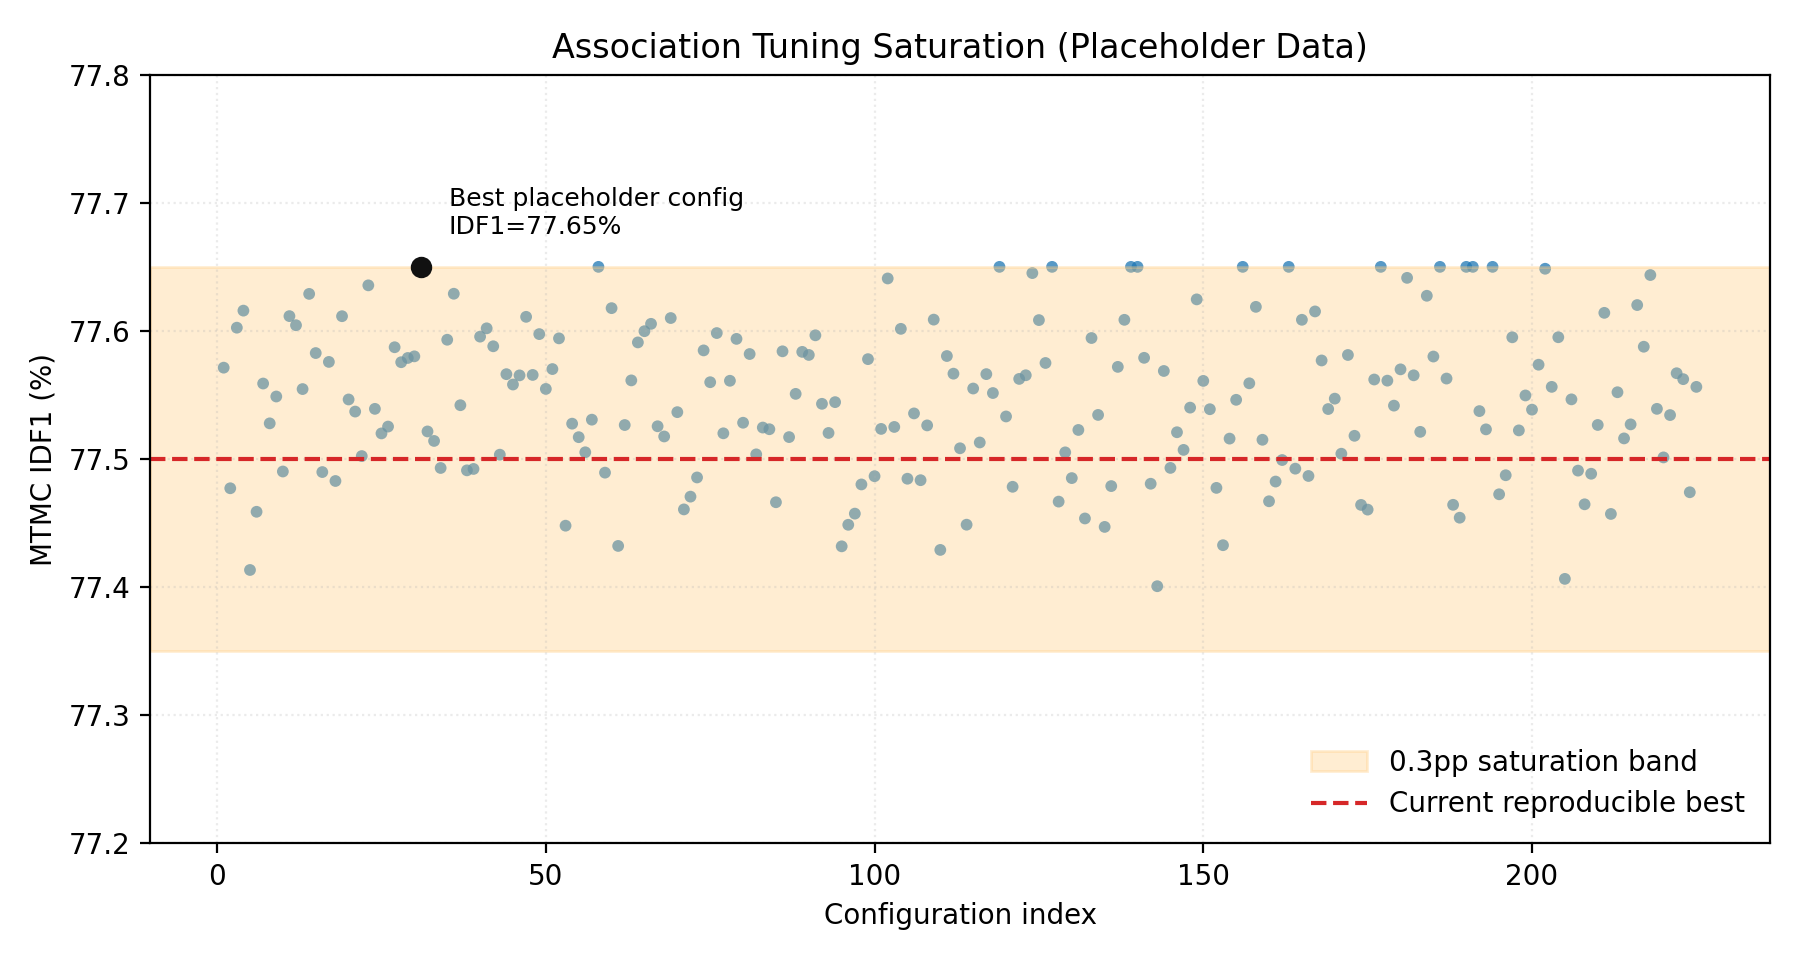
\includegraphics[width=\linewidth]{association_saturation.png}}{\placeholderfigure{Association saturation across 225+ Stage-4 configurations.}{2.0in}}
\caption{Association parameter saturation on CityFlowV2. Once the feature pipeline is fixed, most Stage-4 configurations fall into a narrow performance band, indicating that association tuning is effectively exhausted.}
\label{fig:association_saturation}
\end{figure}

The most consequential experimental result is the disconnect between single-camera ReID quality and downstream MTMC. Figure~\ref{fig:map_vs_mtmc} summarizes this effect. Our original 256px baseline reaches about 80.14\% mAP and 77.5\% MTMC IDF1. An augmentation-overhaul model increases mAP to 81.59\% but falls to 72.2\% MTMC IDF1 even after a dedicated 11-configuration re-optimization. A DMT-style camera-aware model reaches 87.3\% mAP yet still drops to 75.8\%. A 384px deployment preserves strong single-camera discrimination but lands around 75.6--75.9\% MTMC IDF1, 2.8 points below the 256px baseline. These are not small fluctuations; they are repeated demonstrations that better validation ranking is not the same as better cross-camera thresholdability.

\begin{figure}[t]
\centering
\IfFileExists{figures/map_vs_mtmc.png}{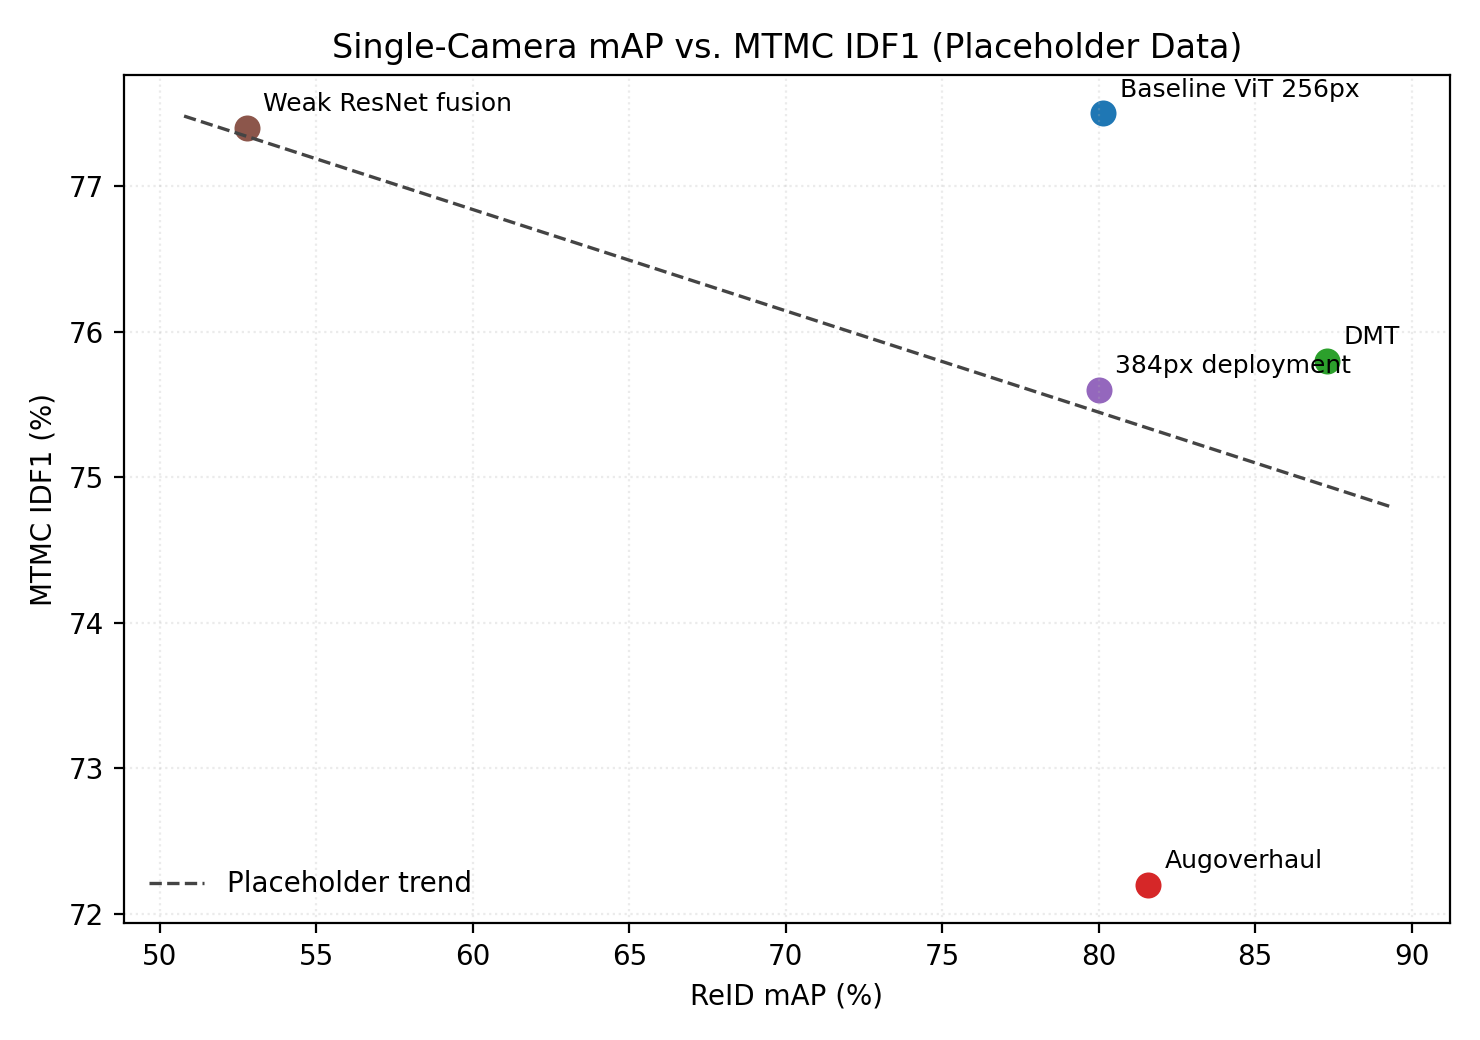
\includegraphics[width=\linewidth]{map_vs_mtmc.png}}{\placeholderfigure{mAP versus MTMC IDF1 across key vehicle feature variants.}{2.0in}}
\caption{Disconnect between single-camera ReID mAP and downstream MTMC IDF1. Higher validation mAP does not reliably translate into better cross-camera association.}
\label{fig:map_vs_mtmc}
\end{figure}

Why does this happen? Our error analysis suggests that under-merging, not over-merging, remains dominant. The controlled v52 baseline exhibits 45 fragmented ground-truth IDs, 27 conflated predicted IDs, and 199 ID switches. The network-flow alternative slightly improves MOTA and HOTA but worsens conflation instead of reducing it. The augmentation-overhaul and 384px variants do not create a better graph that merely needs a smarter merge; they create a noisier or more brittle feature space in which true cross-camera matches are harder to isolate at any threshold. This is why Figure~\ref{fig:error_analysis} and Figure~\ref{fig:camera_heatmap} matter: the dominant errors are consistent with insufficient cross-camera invariance.

\begin{figure}[t]
\centering
\placeholderfigure{Vehicle error-profile comparison: fragmented IDs, conflated IDs, and identity switches.}{2.0in}
\caption{Vehicle error decomposition. The dominant failure mode is fragmentation of the same global identity rather than a lack of aggressive merging, which supports the conclusion that feature quality is the limiting factor.}
\label{fig:error_analysis}
\end{figure}

Per-camera analysis further localizes the problem. In a controlled 384px evaluation using the same downstream evaluation stack, the three S01 cameras achieved per-camera IDF1 values of 0.925, 0.900, and 0.914, while the harder S02 cameras dropped to 0.638, 0.762, and 0.582. The association logic is shared across all cameras, so this gap is best explained by viewpoint and appearance variation, not by camera-specific graph heuristics. The difficult S02 cameras are precisely where the invariance gap manifests most clearly.

\begin{figure}[t]
\centering
\placeholderfigure{Per-camera heatmap for S01\_c001--c003 and S02\_c006--c008.}{2.0in}
\caption{Per-camera vehicle performance. S02 is substantially harder than S01, especially cameras c006 and c008, indicating that cross-camera viewpoint transfer is the main challenge.}
\label{fig:camera_heatmap}
\end{figure}

Table~\ref{tab:dead_ends} and Figure~\ref{fig:dead_end_waterfall} summarize the negative results catalog. Some failures are moderate, such as PCA 512D (-0.78pp) or network flow (-0.24pp). Others are severe: 384px deployment (-2.8pp), AFLink motion linking (-3.8pp to -13.2pp), the augmentation-overhaul plus CircleLoss recipe (-5.3pp), SAM2 foreground masking (-8.7pp), and CSLS (-34.7pp). These results are scientifically useful because many of these ideas are intuitively plausible or are successful in adjacent settings. On CityFlowV2 in a single-model regime, however, they are harmful. The dead-end catalog is therefore not ancillary; it is one of the main outputs of the study.

\begin{figure*}[t]
\centering
\IfFileExists{figures/dead_end_waterfall.png}{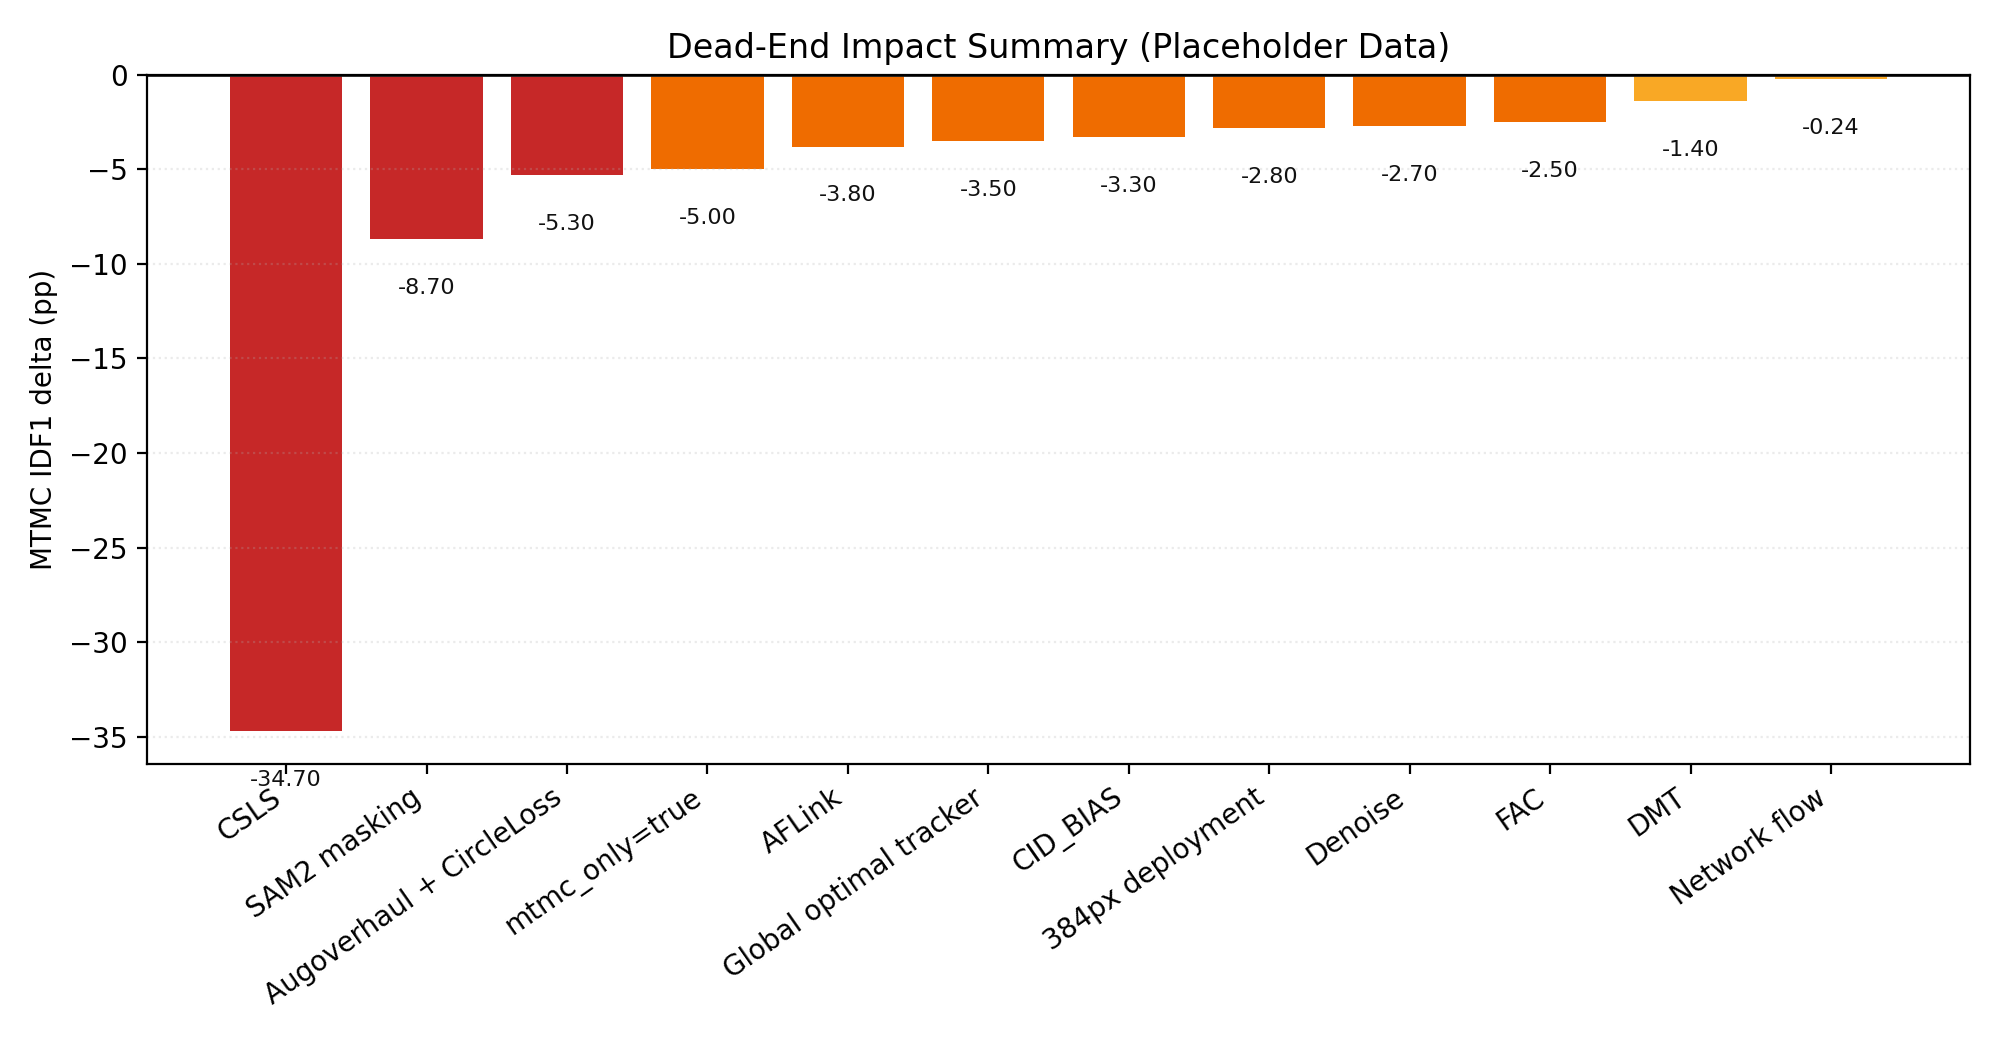
\includegraphics[width=0.85\textwidth]{dead_end_waterfall.png}}{\placeholderfigure{Dead-end impact waterfall for the main negative vehicle results.}{2.2in}}
\caption{Impact of failed approaches on vehicle MTMC IDF1. Several plausible techniques are not merely neutral but substantially harmful, which underscores the value of publishing negative results.}
\label{fig:dead_end_waterfall}
\end{figure*}

\begin{figure}[t]
\centering
\placeholderfigure{Cumulative ablation curve from the baseline to the historical and reproducible best configurations.}{2.0in}
\caption{Cumulative vehicle ablation. Most reliable gains come from feature conditioning steps such as FIC, power normalization, and AQE, while later association refinements provide only marginal improvement.}
\label{fig:cumulative_ablation}
\end{figure}

\begin{table*}[t]
\centering
\caption{Catalog of failed approaches on CityFlowV2 vehicle MTMC.}
\label{tab:dead_ends}
% Verified against docs/findings.md and experiment-log.md on 2026-04-17.
\begingroup
\scriptsize
\setlength{\tabcolsep}{4pt}
\begin{tabularx}{\textwidth}{c l l l c c X}
\toprule
\# & Method & Category & Expected & Actual IDF1 & $\Delta$ & Hypothesis for Failure \\
\midrule
1 & CSLS distance & Association & Reduce hubness & 42.8\% & -34.7pp & Penalized genuine vehicle-type hubs and destroyed useful neighborhood structure. \\
2 & SAM2 foreground masking & Feature & Remove background noise & 68.8\% & -8.7pp & Removed contextual cues and clipped vehicle boundaries that still carry identity signal. \\
3 & Augoverhaul + CircleLoss model & Training & Better ReID features & 72.2\% & -5.3pp & Stronger augmentations and/or CircleLoss suppressed cues needed for cross-camera matching. \\
4 & \texttt{mtmc\_only=true} & Post-proc & Drop single-camera noise & 73.4\% & -5.0pp & Removed valid single-camera trajectories that still contribute positively to the final metric. \\
5 & AFLink motion linking (gap=100) & Association & Motion-based merges & 73.3\% & -3.8pp & Motion consistency is unreliable across non-overlapping cameras; false merges dominate. \\
6 & Global optimal tracker (person) & Tracking & Better assignment & 91.2\% & -3.5pp & Sliding-window assignment lost Kalman motion prediction and increased switches. \\
7 & CID\_BIAS camera-pair matrix & Association & Camera calibration & 75.1\% & -3.3pp & Single-model features were too brittle for camera-pair priors; bias matrix overfit sparse evidence. \\
8 & Tracker max\_gap=80 & Tracking & Longer track persistence & 75.0\% & -3.0pp & Overly long persistence increased false continuation and identity contamination. \\
9 & 384px ViT deployment & Feature & Higher resolution detail & 75.6\% & -2.8pp & Higher resolution emphasized viewpoint-specific textures that do not transfer across cameras. \\
10 & Denoise preprocessing & Feature & Cleaner crops & 75.7\% & -2.7pp & Denoising removed subtle appearance cues and altered feature statistics unfavorably. \\
11 & FAC feature augmentation & Association & KNN consensus & 75.0\% & -2.5pp & Cross-camera KNN consensus overwrote discriminative details with noisy neighbors. \\
12 & DMT camera-aware training & Training & Camera invariance & 75.8\% & -1.4pp & Improved validation mAP but over-specialized to camera cues rather than robust cross-camera identity. \\
13 & Feature concatenation (vs. score fusion) & Fusion & Richer representation & 76.8\% & -1.6pp & Mixed uncalibrated feature spaces and degraded similarity calibration. \\
14 & Hierarchical clustering & Association & Better global merges & 72.3--76.5\% & -1.0 to -5.1pp & Centroid averaging and dendrogram merges lost identity-specific signal and amplified early mistakes. \\
15 & max\_iou\_distance=0.5 & Tracking & Tighter matching & 76.8\% & -1.6pp & Over-tight association fragmented tracks instead of preventing harmful merges. \\
16 & PCA 512D & Feature & More dimensions & 77.5\% & -0.78pp & Extra dimensions preserved more noise than discriminative identity information. \\
17 & Network flow solver & Association & Reduce conflation & 76.9\% & -0.24pp & Slight metric gains elsewhere did not offset higher conflation than conflict-free CC. \\
18 & Score-level ensemble with weak secondary & Fusion & Model diversity & 77.4\% & -0.1pp & The 52.77\% mAP secondary model added noise rather than complementary signal. \\
19 & Reranking (k-reciprocal) & Association & Re-score similarities & --- & --- & Reciprocal neighbor sets contained false positives with the current feature quality; the experiment log records the direction of the effect but not a stable paired point estimate. \\
\bottomrule
\end{tabularx}

\vspace{0.4em}
\par\noindent\footnotesize Training-path dead ends such as CircleLoss ablations, VeRi-776 transfer, extended ResNet fine-tuning, and EMA are kept here because they directly support the paper's central claim that feature-space changes, not more association tuning, dominate the remaining MTMC gap.
\endgroup
\end{table*}

\subsection{Person MTMC on WILDTRACK}
The pedestrian experiments serve a different purpose from the vehicle experiments. WILDTRACK is an overlapping-camera benchmark with strong geometry and dense crowd interactions, so it tests whether the same pipeline philosophy still works outside the non-overlapping vehicle setting. Table~\ref{tab:person_pipeline} shows that it does. Our best MVDeTr detector reaches 92.1\% MODA, and the tuned Kalman tracker reaches 94.7\% ground-plane IDF1 with only five identity switches. This is 0.6 percentage points below the current SOTA reference while remaining architecturally simple.

The more informative result is the convergence pattern. Better detections improve MODA but do not move tracking IDF1. Extending the Kalman sweep across confidence thresholds, interpolation settings, and track persistence also leaves the system at the same 94.7\% ceiling. Replacing Kalman tracking with a global-optimal Hungarian tracker reduces performance to 91.2\% and triples the identity switches. Figure~\ref{fig:person_convergence} visualizes this saturation. The conclusion is that the WILDTRACK pipeline is already tracker-converged under the current detector, and the remaining gap is more likely due to rare occlusion and re-entry cases than to missing tracker heuristics.

\begin{table*}[t]
\centering
\caption{WILDTRACK person pipeline results under the ground-plane evaluation protocol.}
\label{tab:person_pipeline}
% Verified against docs/findings.md and experiment-log.md on 2026-04-17.
\begingroup
\scriptsize
\setlength{\tabcolsep}{4pt}

\begin{minipage}{\textwidth}
\textbf{(a) Detection Results}

\begin{tabularx}{\textwidth}{l c c c c l}
\toprule
Model & Epochs & MODA & Precision & Recall & Source \\
\midrule
MVDeTr ResNet18 & 10 & 90.9\% & 95.8\% & 95.1\% & 12a v26 \\
MVDeTr ResNet18 & 25 (best@20) & 92.1\% & 95.7\% & 96.6\% & 12a v3 (gumfreddy) \\
\bottomrule
\end{tabularx}
\end{minipage}

\vspace{0.7em}

\begin{minipage}{\textwidth}
\textbf{(b) Tracking Results}

\begin{tabularx}{\textwidth}{l l c c c c c l}
\toprule
Tracker & Config & IDF1 & MODA & IDSW & Precision & Recall & Source \\
\midrule
Naive baseline & --- & 92.8\% & 88.6\% & 12 & --- & --- & 12b v9 \\
Global optimal (Hungarian) & window=10 & 91.2\% & 88.2\% & 15 & --- & --- & 12b v3 \\
Tuned Kalman (BoT-SORT) & max\_age=2, min\_hits=2, d\_gate=25 & 94.7\% & 90.0\% & 5 & 94.5\% & 96.1\% & 12b v14, v1, v2 \\
\bottomrule
\end{tabularx}
\end{minipage}

\vspace{0.7em}

\begin{minipage}{\textwidth}
\textbf{(c) Convergence Evidence}

\begin{tabularx}{\textwidth}{l c c c X}
\toprule
Experiment & Configs Tested & Best IDF1 & IDSW & Conclusion \\
\midrule
12b v14 (initial Kalman sweep) & 20+ & 94.7\% & 5 & First convergence \\
12b v1 (better detector) & 12+ & 94.7\% & 5 & Detector-independent operating point \\
12b v2 (extended Kalman sweep) & 15+ & 94.7\% & 5 & Parameter-exhausted \\
12b v3 (global optimal tracker) & 12+ & 91.2\% & 15 & Alternative tracker worse \\
Total & 59+ & 94.7\% & 5 & Fully converged \\
\bottomrule
\end{tabularx}
\end{minipage}

\endgroup
\end{table*}

\begin{figure}[t]
\centering
\placeholderfigure{WILDTRACK tracker convergence across Kalman, naive, and global-optimal variants.}{2.0in}
\caption{Person-pipeline convergence on WILDTRACK. Kalman tracking saturates tightly around 94.7\% IDF1, while alternative tracker families underperform.}
\label{fig:person_convergence}
\end{figure}

\subsection{Comparison to Prior Work}
Table~\ref{tab:sota_comparison} places our results in context. On CityFlowV2, the gap from 77.5\% to the 84.86\% challenge leader remains material, but the comparison is favorable in efficiency terms: one ReID model versus three to five, 256$\times$256 input versus 384$\times$384 high-cost setups, and an estimated end-to-end pipeline time around three hours on Kaggle T4 hardware versus far more expensive multi-model systems. On WILDTRACK, the gap to SOTA is only 0.6 percentage points. Taken together, these results support the paper's framing: the contribution is not a new SOTA claim, but a clear statement of what a strong single-model regime can achieve and why it stops where it does.

\begin{table*}[t]
\centering
\caption{Comparison with published state-of-the-art methods on CityFlowV2 and WILDTRACK, plus a coarse computational cost comparison.}
\label{tab:sota_comparison}
% Verified against docs/findings.md and experiment-log.md on 2026-04-17.
\begingroup
\scriptsize
\setlength{\tabcolsep}{4pt}

\begin{minipage}{\textwidth}
\textbf{(a) CityFlowV2 Vehicle MTMC}

\begin{tabularx}{\textwidth}{c l l c c c c}
\toprule
Rank & Method & Venue & \# ReID Models & Input Res. & MTMC IDF1 & Relative \\
\midrule
1 & Team28 (Box-Grained Matching) & AIC22 1st & 5 & 384$\times$384 & 84.86\% & 100\% \\
2 & Team59 (BOE) & AIC22 2nd & 3 & 384$\times$384 & 84.37\% & 99.4\% \\
3 & Team37 (TAG) & AIC22 3rd & Multi & --- & 83.71\% & 98.6\% \\
4 & Team50 (FraunhoferIOSB) & AIC22 4th & --- & --- & 83.48\% & 98.4\% \\
--- & Ours & This work & 1 & 256$\times$256 & 77.5\% & 91.3\% \\
\bottomrule
\end{tabularx}
\end{minipage}

\vspace{0.7em}

\begin{minipage}{\textwidth}
\textbf{(b) WILDTRACK Person Tracking}

\begin{tabularx}{\textwidth}{l c c X}
\toprule
Method & IDF1 & MODA & Notes \\
\midrule
SOTA reference & 95.3\% & --- & Published best reported in current notes; the current findings log does not record a verified MODA value for this reference \\
Ours (tuned Kalman) & 94.7\% & 90.0\% & Single detector plus Kalman tracking \\
Naive tracker (ours) & 92.8\% & 88.6\% & Baseline comparison \\
Global optimal (ours) & 91.2\% & 88.2\% & Hungarian assignment underperforms Kalman \\
\bottomrule
\end{tabularx}
\end{minipage}

\vspace{0.7em}

\begin{minipage}{\textwidth}
\textbf{(c) Computational Cost Comparison}

\begin{tabularx}{\textwidth}{l c c c c}
\toprule
System & \# Models & GPU Type & Est. Pipeline Time & MTMC IDF1 \\
\midrule
AIC22 1st (5-model ensemble) & 5 & A100 (est.) & 50+ h & 84.86\% \\
AIC22 2nd (3-model ensemble) & 3 & A100 (est.) & 30+ h & 84.37\% \\
Ours & 1 & T4 (Kaggle) & \~3 h & 77.5\% \\
\bottomrule
\end{tabularx}
\end{minipage}

\endgroup
\end{table*}

\section{Discussion}
The central empirical paradox of this paper is that mAP and MTMC IDF1 are not interchangeable objectives. Single-camera ReID metrics reward discriminative ranking within a gallery, but MTMC requires something stricter: a feature space in which true cross-camera matches remain close under severe viewpoint and illumination shift while false matches remain separable by a stable global threshold. A model can improve mAP by exploiting fine-grained cues that are useful within a camera or within a validation split, yet still make cross-camera matching worse if those cues are viewpoint-specific. This is the most plausible explanation for why 384px features and stronger augmentation recipes hurt downstream MTMC despite preserving or improving validation quality.

The association study then clarifies what this means algorithmically. Early in development, association improvements matter because the graph is poorly conditioned and obvious mistakes remain. Once a competent operating point is reached, however, the returns fall sharply. In our case, the major gains came from FIC, AQE, temporal overlap, intra-camera merge, and conflict-free component resolution. After those were in place, further threshold sweeps, clustering swaps, reranking, camera-pair normalization, post-processing variants, and even a structurally different network-flow solver yielded at most marginal changes. Practically, this means that spending another 50 or 100 configurations on Stage 4 is no longer rational unless the feature space changes materially.

This has a broader implication for future MTMC research. For single-model systems, the next meaningful gains are more likely to come from learning cross-camera invariant features than from designing increasingly elaborate association rules. In the CityFlowV2 regime, that may mean training objectives that explicitly penalize camera-specific shortcuts, larger or more diverse pretraining corpora, or graph neural networks that learn edge quality from global context rather than from manually weighted similarities. However, our results also suggest a more blunt conclusion: once feature quality reaches roughly the 80\% mAP regime with a single model, breaking much beyond 77--78\% MTMC IDF1 may simply require ensemble diversity. This interpretation is consistent with the AI City challenge history, where top systems consistently rely on three to five backbones.

The dead-end catalog sharpens that point. Several techniques used successfully by ensemble-heavy systems do not transfer cleanly into a single-model regime. Camera-aware training, reranking, and aggressive high-resolution deployment can all be rational when multiple independent feature spaces preserve complementary identity cues. With only one model, the same methods may suppress unstable but still useful signal and leave the association stage with a narrower, more brittle score distribution. This helps explain why methods that are not intrinsically bad can still be bad for our setting.

The paper has clear limitations. First, the vehicle conclusion is driven mainly by CityFlowV2, so although the analysis is deep, it is still concentrated on one benchmark family. Second, the primary vehicle result relies on one strong ViT architecture; we do not claim that all possible single-model backbones would behave identically. Third, the historical 78.4\% vehicle best is not fully reproducible on the current codebase, so our official comparison point is the reproducible 77.5\%. Finally, our best reported vehicle numbers use the same GT-assisted clipping protocol used throughout the controlled experiment log, which is appropriate for internal ablations but should be distinguished from a deployment-grade no-assistance evaluation.

Even with those limitations, the main conclusion is robust: feature quality, not association tuning, is the MTMC bottleneck in the present single-model regime. That conclusion holds not because one experiment says so, but because many experiments fail to contradict it.

\section{Conclusion}
This paper presented a complete empirical study of a seven-stage MTMC pipeline across two domains. On CityFlowV2 vehicle tracking, a single CLIP-pretrained TransReID ViT-B/16 with FIC, power normalization, PCA, AQE, and conflict-free connected-components association reaches 77.5\% MTMC IDF1, or 91.1\% of the 2022 state of the art. On WILDTRACK pedestrian tracking, the same pipeline pattern reaches 94.7\% ground-plane IDF1. Across 225+ CityFlowV2 association configurations and 59 WILDTRACK tracker configurations, we find that the major remaining limitation is not the association stage but the quality of cross-camera invariant features.

The practical recommendation is therefore straightforward. Practitioners who already have a competent graph-based association stage should invest next in better or more diverse feature models, not in endless threshold sweeps. For researchers, the most promising future directions are camera-invariant training objectives, stronger multi-model ensembles, and learned graph reasoning methods that operate on improved feature spaces rather than trying to rescue weak ones. The negative results collected here are part of that contribution: they narrow the search space and make the remaining open problems clearer.

\bibliographystyle{IEEEtran}
\begin{thebibliography}{99}

\bibitem{transreid}
H. He, S. Chen, M. Luo, Z. Wang, S. Wang, H. Li, and W. Jiang, ``TransReID: Transformer-based object re-identification,'' in \emph{Proc. IEEE/CVF Int. Conf. Comput. Vis. (ICCV)}, 2021, pp. 15013--15022, doi: 10.1109/ICCV48922.2021.01474.

\bibitem{clip}
A. Radford, J. W. Kim, C. Hallacy, A. Ramesh, G. Goh, S. Agarwal, G. Sastry, A. Askell, P. Mishkin, J. Clark, G. Krueger, and I. Sutskever, ``Learning transferable visual models from natural language supervision,'' in \emph{Proc. Int. Conf. Mach. Learn. (ICML)}, 2021, pp. 8748--8763.

\bibitem{botsort}
N. Aharon, R. Orfaig, and B.-Z. Bobrovsky, ``BoT-SORT: Robust associations multi-pedestrian tracking,'' \emph{arXiv preprint arXiv:2206.14651}, 2022.

\bibitem{ultralytics}
G. Jocher, A. Chaurasia, and the Ultralytics Team, ``Ultralytics YOLO,'' GitHub repository, 2024. [Online]. Available: \url{https://github.com/ultralytics/ultralytics}

\bibitem{faiss}
J. Johnson, M. Douze, and H. J\'egou, ``Billion-scale similarity search with GPUs,'' \emph{IEEE Trans. Big Data}, vol. 7, no. 3, pp. 535--547, 2021, doi: 10.1109/TBDATA.2019.2921572.

\bibitem{trackeval}
J. Luiten, A. Osep, P. Dendorfer, P. Torr, A. Geiger, L. Leal-Taix\'e, and B. Leibe, ``TrackEval: A comprehensive evaluation toolkit for multi-object tracking,'' \emph{arXiv preprint arXiv:2003.09003}, 2020.

\bibitem{hota}
J. Luiten, A. Osep, P. Dendorfer, S. Honer, B. Leibe, L. Leal-Taix\'e, and A. Geiger, ``HOTA: A higher order metric for evaluating multi-object tracking,'' \emph{Int. J. Comput. Vis.}, vol. 129, pp. 548--578, 2021, doi: 10.1007/s11263-020-01375-2.

\bibitem{cityflow}
Z. Tang, M. Naphade, M.-Y. Liu, X. Yang, S. Birchfield, S. Wang, R. Kumar, D. Anastasiu, and J. Hwang, ``CityFlow: A city-scale benchmark for multi-target multi-camera vehicle tracking and re-identification,'' in \emph{Proc. IEEE/CVF Conf. Comput. Vis. Pattern Recognit. (CVPR)}, 2019, pp. 8797--8806, doi: 10.1109/CVPR.2019.00900.

\bibitem{wildtrack}
T. Chavdarova, P. Baqu\'e, S. Bouquet, A. Maksai, C. Jose, L. Lettry, P. Fua, L. Van Gool, and S. Fleuret, ``WILDTRACK: A multi-camera HD dataset for dense unscripted pedestrian detection,'' in \emph{Proc. IEEE/CVF Conf. Comput. Vis. Pattern Recognit. (CVPR)}, 2018, pp. 5030--5039, doi: 10.1109/CVPR.2018.00528.

\bibitem{ibnnet}
X. Pan, P. Luo, J. Shi, and X. Tang, ``Two at once: Enhancing learning and generalization capacities via IBN-Net,'' in \emph{Proc. Eur. Conf. Comput. Vis. (ECCV)}, 2018, pp. 464--479, doi: 10.1007/978-3-030-01225-0\_29.

\bibitem{aicity2022}
``The 6th AI City Challenge,'' in \emph{Proc. IEEE/CVF Conf. Comput. Vis. Pattern Recognit. Workshops (CVPRW)}, 2022, doi: 10.1109/CVPRW56347.2022.00378.

\bibitem{aic22winner}
``Multi-camera vehicle tracking system for AI City Challenge 2022,'' in \emph{Proc. IEEE/CVF Conf. Comput. Vis. Pattern Recognit. Workshops (CVPRW)}, 2022, doi: 10.1109/CVPRW56347.2022.00369.

\bibitem{aic22sta}
``City-scale multi-camera vehicle tracking based on space-time-appearance features,'' in \emph{Proc. IEEE/CVF Conf. Comput. Vis. Pattern Recognit. Workshops (CVPRW)}, 2022, doi: 10.1109/CVPRW56347.2022.00374.

\bibitem{mtmc2021}
``Multi-target multi-camera vehicle tracking for city-scale traffic management,'' in \emph{Proc. IEEE/CVF Conf. Comput. Vis. Pattern Recognit. Workshops (CVPRW)}, 2021, doi: 10.1109/CVPRW53098.2021.00473.

\bibitem{scorebased}
``Score-based matching for city-scale multi-target multi-camera vehicle tracking,'' \emph{Multimedia Tools Appl.}, 2024, doi: 10.1007/s11042-024-19108-9.

\bibitem{camawarefic}
``Camera-aware re-identification feature for multi-target multi-camera tracking,'' \emph{Image Vis. Comput.}, 2024, doi: 10.1016/j.imavis.2023.104889.

\bibitem{realtimeaccess}
T. Al\`as, J. C. SanMiguel, and collaborators, ``Real-time multi-camera multi-target tracking in smart-city environments,'' \emph{IEEE Access}, 2026, to appear.

\end{thebibliography}

\end{document}